\documentclass[11pt,aspectratio=169]{beamer}
%%%%%%%%% GENERAL PACKAGES
%\usepackage[dvipsnames]{xcolor}
%\usepackage{pdfpages}
%\usetheme[progressbar=frametitle]{metropolis}
%\setbeamercolor{background canvas}{bg=white}
%\usepackage{appendixnumberbeamer}
%\usepackage{booktabs}
%\usepackage[scale=2]{ccicons}
%\usepackage{pgfplots}
%\usepgfplotslibrary{dateplot}
%\usepackage{xspace}
%\newcommand{\themename}{\textbf{\textsc{metropolis}}\xspace}
%\usepackage[absolute,overlay]{textpos}






%%%%%%%%% COLOR THEME

% Define some colors:
\definecolor{DarkFern}{HTML}{407428}
\definecolor{DarkCharcoal}{HTML}{4D4944}
\definecolor{AlertColor}{RGB}{89,124,158}
\definecolor{HighLight}{RGB}{96,95,134}
\definecolor{Important}{RGB}{234,122,133}
\definecolor{Yellow}{HTML}{00539C}
\colorlet{Fern}{DarkFern!85!white}
\colorlet{Charcoal}{DarkCharcoal!85!white}
\colorlet{LightCharcoal}{Charcoal!50!white}
\colorlet{HighLight2}{AlertColor}
\colorlet{DarkRed}{red!70!black}
\colorlet{DarkBlue}{blue!70!black}
\colorlet{DarkGreen}{green!70!black}
\definecolor{RoyalBlue}{HTML}{00539C}
\definecolor{Peach}{HTML}{EEA47F}
\definecolor{ForestGreen}{HTML}{2C5F2D}
\definecolor{MossGreen}{HTML}{E8FCC9}
\definecolor{SeaGreen}{HTML}{2E8B57}
% Use the colors:
\setbeamercolor{title}{fg=Fern}
\setbeamercolor{frametitle}{fg=MossGreen,bg=ForestGreen}
\setbeamercolor{normal text}{fg=Charcoal!70!black}
\setbeamercolor{block title}{fg=black,bg=Fern!25!white}
\setbeamercolor{block body}{fg=black,bg=Fern!10!white}
\setbeamercolor{block title alerted}{fg=black,bg=DarkRed!25!white}
\setbeamercolor{block body alerted}{fg=black,bg=DarkRed!10!white}
\setbeamercolor{alerted text}{fg=DarkRed}
\setbeamercolor{itemize item}{fg=Charcoal}



%%%%%%%%% OTHER COMMANDS
\newcommand{\indep}{\perp\!\!\! \perp}
\newcommand{\comment}[1]{}
\newcommand{\bs}{\boldsymbol}
\newcommand{\tr}{\text{trace}}
\newcommand{\sgn}{{\rm sgn}}
\def\T{\top}
%\newcommand{\det}{\text{det}}
\newcommand{\var}{\mathrm{var}}
\newcommand{\cC}{{\cal C}}
\renewcommand{\d}{{\rm d}}
\newcommand{\cG}{{\cal G}}
\newcommand{\cV}{{\cal V}}
\newcommand{\cE}{{\cal E}}
\newcommand{\cM}{{\cal M}}
\newcommand{\cP}{{\cal P}}
\newcommand{\cX}{{\cal X}}
\newcommand{\cY}{{\cal Y}}
\newcommand{\X}{\mathbf{X}}
\newcommand{\Y}{\mathbf{Y}}
\newcommand{\x}{\mathbf{x}}
\newcommand{\y}{\mathbf{y}}
\newcommand{\z}{\mathbf{z}}

\newcommand{\argmin}{\operatornamewithlimits{argmin}}
\newcommand{\eps}{\varepsilon}
\newcommand{\<}{\langle}
\renewcommand{\>}{\rangle}


%

\setbeamertemplate{navigation symbols}{}
\setbeamertemplate{footline}[text line]{%
    \hfill\strut{%
        \scriptsize\sf\color{black!60}%
        \quad\insertframenumber/\inserttotalframenumber
    }
    %\hfill
    }


\usenavigationsymbolstemplate{}
\setbeamersize{text margin left=.2cm,text margin right=.2cm} 
\addtobeamertemplate{frametitle}{}{\vspace{-1.2mm}}
\setbeamertemplate{itemize item}{$\bullet$}

\setbeamertemplate{itemize subitem}{\tiny\raise1.5pt\hbox{\donotcoloroutermaths$\blacktriangleright$}}
\setbeamertemplate{itemize subsubitem}{\tiny\raise1.5pt\hbox{\donotcoloroutermaths$\blacktriangleright$}}
\setbeamertemplate{enumerate item}{\insertenumlabel.}
\setbeamertemplate{enumerate subitem}{\insertenumlabel.\insertsubenumlabel}
\setbeamertemplate{enumerate subsubitem}{\insertenumlabel.\insertsubenumlabel.\insertsubsubenumlabel}
\setbeamertemplate{enumerate mini template}{\insertenumlabel}






\newcommand{\TODO}[1]{{\color{red}{[TODO: #1]}}}


\newcommand{\R}{\mathbb R}
\newcommand{\E}{\mathbb E}
\renewcommand{\P}{\mathbb P}


\DeclareMathOperator*{\cov}{cov}


\newsavebox{\zerobox}
\newenvironment{nospace}
{\par\edef\theprevdepth{\the\prevdepth}\nointerlineskip
  \setbox\zerobox=\vtop to 0pt\bgroup
  \hrule height0pt\kern\dimexpr\baselineskip-\topskip\relax
}
{\par\vss\egroup\ht\zerobox=0pt \wd\zerobox=0pt \dp\zerobox=0pt
  \box\zerobox}

\usepackage{soul}
\makeatletter
\let\HL\hl
\renewcommand\hl{%
  \let\set@color\beamerorig@set@color
  \let\reset@color\beamerorig@reset@color
  \HL}
  \makeatother



%\usecolortheme{whale}

\title[Calculus and Linear Algebra]{Lecture 2 : Calculus and Linear Algebra}
\author[Piotr Zwiernik, Barcelona School of Economics]{Piotr Zwiernik \\ $\;$\\
Mathematics Brush-up\\ $\;$\\ $\;$\\

\includegraphics[width=1.5in]{img/bse.png}  
}
\date{}


%\beamerdefaultoverlayspecification{<+->}

\begin{document}
\begin{frame}
\titlepage
\end{frame}



%--------------- slide 2  ----------------%



\begin{frame}{Chapter 4: Integration}

Often, a function $f$ is given, and we are looking for \hl{$F$ whose derivative is $f$}.
\vskip 12pt
\textcolor{blue}{Example:} the marginal cost function $C'$ is given (we know how cost changes according the production), and we want to find $C$.
\vskip 12pt
$F$ can be found by \textcolor{blue}{integration}, which is the reverse process of differentiation.
\vskip 12pt
\textcolor{blue}{Read}  Chapter 5 of Werner-Sotskov 
\vskip 12pt
\textcolor{blue}{Exercises:} 5.1 (a)-(b), 5.2 (a)-(b), 5.3 (c) (Werner-Sotskov)
\end{frame}
\begin{frame}{Indefinite integrals}

A differentiable function $F$ is called an \textcolor{blue}{antiderivative} of a function $f$ if $F'(x)=f(x)$, for all $x \in D_F=D_f$.
\vskip 12pt
\textcolor{blue}{Theorem:} Then, all antiderivatives of $f$ are of the form $\tilde{F}(x)=F(x)+c$ where $c$ is any constant.
\vskip 12pt
The \textcolor{blue}{indefinite integral} of $f$ is defined as $$\int f(x) dx=F(x)+c$$

\textcolor{blue}{Properties (integration is a linear operation):}
\begin{enumerate}
\item $\int (f(x)+g(x)) dx=\int f(x) dx+\int g(x) dx$.
\item $\int cf(x) dx= c \int f(x) dx$.
\end{enumerate}\end{frame}

\begin{frame}{Indefinite integrals}
\textcolor{blue}{Some indefinite integrals:}
\begin{enumerate}
\item $\int x^n dx =\frac{x^{n+1}}{n+1} +c$, $n \neq -1$  \\[3mm]
\item $\int \frac{1}{x} dx=\log \vert x \vert +c$ \\[3mm]
\item $\int e^x dx= e^x +c$.\\[3mm]
\item $\int \sin(x) dx=-\cos(x)+c \qquad $\\[3mm]
\item $\int \cos(x) dx=\sin(x)+c$\\[3mm]
\item $\int a^x dx=\frac{a^x}{\log a} +c, a>0, a \neq 1$\\[3mm]
\end{enumerate}
\begin{small} Proof: differentiate the right hand side to obtain the expression  inside the integral \end{small}
\end{frame}

\begin{frame}{Integration by substitution}
\begin{block}{Theorem (Integration by substitution)}
Assume that $f$ has an antiderivative $F$, and let $g$  continuously differentiable.
Then setting $t=g(x)$, we obtain 
$$
\int f(g(x)) g'(x) dx=\int f(t) dt=F(t)+c=F(g(x))+c.
$$	
\end{block}
 \textcolor{blue}{Examples:}
$$
1. \int (ax+b)^n dx= \frac{1}{a} \int t^n dt=\frac{t^{n+1}}{a(n+1)}+c=\frac{(ax+b)^{n+1}}{a(n+1)}+c 
$$

\begin{tiny} ($t=ax+b, dt=adx$)\end{tiny}

$$
2. \int \frac{e^x}{\sqrt[3]{1+e^x}} dx=\int t^{-1/3} dt=\frac{3}{2} t^{2/3}+c=
\frac32 (1+e^x)^{2/3}+c 
$$
 \begin{tiny} ($t=1+e^x, dt=e^x dx$)\end{tiny}
\end{frame}

\begin{frame}{Integration by parts}
\begin{block}{Theorem (Integration by parts)}
Let $u,v$ two differentiable functions. Then
$$
 \int u(x)v'(x) dx=u(x)v(x)- \int u'(x)v(x) dx.
$$	
\vspace{-5mm}\begin{tiny}Proof: Apply the product  rule to $(u(x)v(x))'$ and integrate. \end{tiny}
\end{block}
\bigskip 

\textcolor{blue}{Example:} Apply the theorem with $u=\log(x), v'=1$ to get 
	$$
\int \log x dx=x \log x-\int dx=x(\log x -1) +c 
 $$
 \end{frame}

\begin{frame}{Another example}
First integrate by substitution $\sqrt{x}=t, 2 \sqrt{x} dt=dx$ then integrate by parts with $u=t, v'=\sin t$ to get
\begin{equation*} \begin{split}
&\int \sin \sqrt{x} dx=2 \int t \sin t \, dt= 2 (-t\cos t +\int \cos t \, dt)\\
&\qquad =2(-t\cos t+\sin t) +c =2(-\sqrt{x} \cos \sqrt{x}+\sin \sqrt{x})+c
 \end{split}
 \end{equation*}	
\end{frame}


\begin{frame}{The definite integral}

The \textcolor{blue}{definite integral} of $f:[a,b] \rightarrow \R_+$ continuous equals the 
\textcolor{blue}{area} covered by the $x$-axis and the graph of $f$.
\vskip 12pt
 \textcolor{blue}{Notation:} $\int_b^a f(x) dx.$ \textcolor{blue}{Remark:} If $f$ is only bounded in $[a,b]$ with at most a finite number of discontinuities, the definite integral always exists.
 




 \textcolor{blue}{Properties:} 
\begin{enumerate}
\item $\int_b^a f(x) dx=- \int_a^b f(x) dx $

\item  $\int_a^b cf(x) dx=c \int_a^b f(x) dx$.

\item If $c \in [a,b]$ then $\int_a^b f(x) dx= \int_a^c f(x) dx +\int_c^b f(x) dx$.
\item $\big\vert \int_a^b f(x) dx\big\vert \leq \int_a^b \vert f(x) \vert dx$.
\item If $f,g$ are continuous in $[a,b]$ and $f(x) \leq g(x)$ for all $x \in [a,b]$, then
$$
\int_a^b f(x) dx\leq \int_a^b g(x) dx.
$$
\end{enumerate}\end{frame}\begin{frame}{The definite integral}

\textcolor{blue}{Theorem:} Let $f$ continuous on $[a,b]$ with antiderivative $F$. Then 
$$
\int_a^b f(x) dx=F(b)-F(a).
$$
Moreover, the function $G(t)=\int_a^t f(x) dx$ is differentiable in $[a,b]$ and
$G'(t)=f(t)$. 
\vskip 12pt

\textcolor{blue}{Example:} The marginal cost of a firm producing one product is
$$
C'(x)=6-\frac{60}{x+1}, \qquad x \in [0,1000].
$$
If the quantity produced changes form 300 to 400, the cost changes by
\begin{equation*}
\begin{split}
C(400)-C(300)&=\int_{300}^{400} C'(x) dx=(6x-60\log \vert x+1 \vert) \bigg\vert_{300}^{400} \\
&\approx 582.79
\end{split}
\end{equation*}
\end{frame}


\begin{frame}{Application of the  integral: Proof of the number $e$}

We can define the \textcolor{blue}{ logarithm function} as
$$
\log x =\int_1^x \frac{1}{t} dt.
$$
We then  define the  \textcolor{blue}{exponential function} $e^x$ as the unique inverse of $\log x$. In particular, $\log e=1$, so $1=\int_1^e \frac{1}{t} dt$.

We are  going to show that $$e=\lim_{n \rightarrow \infty} \left(1+\frac{1}{n} \right)^n.$$

Let  $t \in [1, 1+\frac1n]$. Then
$$
\int_1^{1+\frac1n} \frac{1}{1+\frac1n} dt \leq \int_1^{1+\frac1n} \frac{1}{t} dt \leq \int_1^{1+\frac1n} 1 dt.
$$
Therefore
$$
\frac{1}{n+1} \leq  \log \left(1+\frac1n \right) \leq \frac1n.
$$
\end{frame}


\begin{frame}{Application: Proof of the number $e$}

 Taking the  exponential, we get
$$
e^{\frac{1}{1+n}} \leq 1+\frac1n \leq e^{\frac1n}.
$$
Taking the  $(n+1)th$ power of the  left inequality and the  $nth$ power of the  right, gives
$$
\left(1+\frac{1}{n} \right)^n \leq e \leq \left(1+\frac{1}{n} \right)^{n+1}.
$$

 Divide the  right  inequality by  $1+\frac1n$ and combine with the left inequality  to get
$$
\frac{e}{1+\frac{1}{n} }\leq \left(1+\frac{1}{n} \right)^n \leq e.
$$

Taking the limit as $n \rightarrow \infty$ we obtain the result.
\end{frame}

\begin{frame}{Application of the  integral: Taylor's formula $n=2$}

Applying 3 times the theorem in slide 8, we get
\begin{equation*} \begin{split}
&f(x)=f(x_0)+\int_{x_0}^x f'(t_1) dt_1 \\
&=f(x_0)+\int_{x_0}^x f'(x_0) dt_1+\int_{x_0}^x \int_{x_0}^{t_1} f''(t_2) dt_2 dt_1 \\
&=f(x_0)+\int_{x_0}^x f'(x_0) dt_1+\int_{x_0}^x \int_{x_0}^{t_1} f''(x_0) dt_2 dt_1 +\int_{x_0}^x \int_{x_0}^{t_1} \int_{x_0}^{t_2} f'''(t_3) dt_3  dt_2 dt_1\\
&=f(x_0) +f'(x_0)(x-x_0)+\frac{f''(x_0)}{2}(x-x_0)^2
+\int_{x_0}^x \int_{x_0}^{t_1} \int_{x_0}^{t_2} f'''(t_3) dt_3  dt_2 dt_1
\end{split}
\end{equation*}
Finally, using the intermediate value theorem, we get that there exists $y \in (x_0, x)$ such that
$$
\int_{x_0}^x \int_{x_0}^{t_1} \int_{x_0}^{t_2} f'''(t_3) dt_3  dt_2 dt_1=f'''(y) \frac{(x-x_0)^3}{3!}.
$$\end{frame}

\begin{frame}{Chapter 5: Vectors}

A \textcolor{blue}{vector} is an ordered $n$-tuple
\vskip 12pt
This is important in economics, since it can describe a bundle of commodities such that the $i$th value represents the quantity of the $i$th commodity.
\vskip 12pt
\textcolor{blue}{Read}  Chapter 6 of Werner-Sotskov and Chapters 10 and 11 of Simon-Blume
\vskip 12pt

 \textcolor{blue}{Exercises:} 6.2, 6.3, 6.4, 6.6, 6.7, 6.8 (Werner-Sotskov)
\end{frame}

\begin{frame}{Definition}

A \textcolor{blue}{vector} $\bf{v}=$ is an ordered $n$-tuple of real numbers $v_1,\dots,v_n$ called the \textcolor{blue}{coordinates}, which points a \textcolor{blue}{direction} between two $n$-dimensional points.
\textcolor{blue}{Notation:}
\begin{equation*}
{\bf v}=\begin{pmatrix}v_1\\
v_2 \\
\vdots\\
v_n
\end{pmatrix} \qquad  {\bf v}'=(v_1,\ldots,v_n).
\end{equation*}

The set of all real $n$-tuples is called the $n$-dimensional space $\R^n$: 
\begin{equation*}
\R^n=\left\{\begin{pmatrix}v_1\\
v_2 \\
\vdots\\
v_n
\end{pmatrix}\;  \bigg\vert \; v_i \in \R, i=1,2,\dots,n \right\}
\end{equation*}

Special vectors: the \textcolor{blue}{zero vector} ${\bf 0}'=(0,0,\dots,0)$, and the $i$th \textcolor{blue}{unit vector} ${\bf e_i}'=(0,\dots,0,1,0,\dots,0)$, the 1 is at the $i$th component.
\end{frame}

\begin{frame}{Operations on vectors}

\textcolor{blue}{Sum of two vectors}:
\begin{equation*}
\bf{u}+\bf{v}=\begin{pmatrix}u_1\\
u_2 \\
\vdots\\
u_n
\end{pmatrix}+
\begin{pmatrix}v_1\\
v_2 \\
\vdots\\
v_n
\end{pmatrix}=\begin{pmatrix}u_1+v_1\\
u_2+v_2 \\
\vdots\\
u_n+v_n
\end{pmatrix}.
\end{equation*}

\textcolor{blue}{Multiplication of a vector by a scalar} $\lambda \in \mathbb{R}$:
\begin{equation*}
\lambda \bf{v}=\lambda\begin{pmatrix}v_1\\
v_2 \\
\vdots\\
v_n
\end{pmatrix}=
\begin{pmatrix} \lambda v_1\\
\lambda v_2 \\
\vdots\\
\lambda v_n
\end{pmatrix}.
\end{equation*}

\textcolor{blue}{Difference of two vectors}: $\bf{u}-\bf{v}=\bf{u}+(-1)\bf{v}$.
\vskip 10pt
Theses properties satisfy the usual \textcolor{blue}{distributive, commutative and associative laws}.
\end{frame}

\begin{frame}{Sum and difference of two vectors}

\begin{figure}
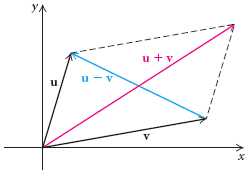
\includegraphics[width=2.5in]{img/sum} 
\end{figure}\end{frame}

\begin{frame}{Scalar or inner product}

The \textcolor{blue}{scalar or inner product} of two vectors ${\bf u}, {\bf v}\in \R^n$ is defined as
$$
{\bf u}' {\bf v}=u_1 v_1+\cdots +u_nv_n.
$$

\textcolor{blue}{Properties:}
\begin{enumerate}
\item Commutative: ${\bf u}' {\bf v}= {\bf v}' {\bf u}$.
\item Distributive: ${\bf u}' ({\bf v}+{\bf  w})={\bf u}' {\bf v}+{\bf u}' {\bf w}$.
\item Not necessarily associative: $\bf{u} ({\bf v}' {\bf w}) \neq ({\bf u}' {\bf v}) {\bf w}$.
\end{enumerate}
\vskip 12pt
\textcolor{blue}{Example:} The total cost of production of a firm that produces the quantities ${\bf u}'=(30,40,10)$ of three products with cost of production ${\bf v}'=(20,15, 40)$ is:
$$
{\bf u}' {\bf v}=20 \cdot 30+15 \cdot 40+ 40 \cdot 10=1600
$$
\end{frame}\begin{frame}{Norm of a vector}

The \textcolor{blue}{norm of a vector} ${\bf v} \in \R^n$ is defined as
$$
\vert {\bf v}\vert=\sqrt{ {\bf v}' {\bf v}}=\sqrt{v_1^2+\dots+v^2_n}.
$$


\textcolor{blue}{Geometric interpretation:} The norm of a vector is its \textcolor{blue}{length} (the distance to ${\bf 0}$). The distance between two vectors 
${\bf u}$ and ${\bf v}$ is defined as $\vert {\bf u}-{\bf v}\vert$. This is the length of the vector connecting the terminal points of ${\bf u}$ and ${\bf v}$.
If  $\vert {\bf v} \vert=1$, then ${\bf v}$ is called a \textcolor{blue}{unit vector}.

\textcolor{blue}{Properties:}
\begin{enumerate}
\item $\vert {\bf v} \vert\geq 0$ and $\vert {\bf v} \vert =0$ if and only if ${\bf v}=\bf{0}$.
\item $\vert \lambda {\bf v} \vert = \vert \lambda \vert \, \vert {\bf v} \vert $ for all $\lambda \in \R.$


\item $
\vert {\bf u}- {\bf v}\vert^2=\vert {\bf u} \vert^2 +\vert {\bf v}\vert^2-2 \vert {\bf u} \vert \, \vert {\bf v}\vert \cos ({\bf u}, {\bf v}).
$ \begin{tiny}Proof: use the  Law of Cosines \end{tiny}


\item ${\bf u}' {\bf v} = \vert {\bf u}\vert \, \vert {\bf v} \vert \cos ({\bf u}, {\bf v})$
\begin{tiny}Proof: use 3. and  $\vert {\bf u}- {\bf v}\vert^2=\vert {\bf u} \vert^2 +\vert {\bf v}\vert^2-2 {\bf u}' {\bf v}$. \end{tiny}

\item \textcolor{blue}{Cauchy-Schwarz inequality:} $ {\bf u}' {\bf v} \leq  \vert {\bf u} \vert \, \vert {\bf v} \vert$ \begin{tiny}Proof: use 4.\end{tiny}

\item $\vert {\bf u} +{\bf v}\vert\leq \vert {\bf u}\vert +\vert {\bf v}\vert$. \begin{tiny}Proof: use 5. and $\vert {\bf u}+ {\bf v}\vert^2=\vert {\bf u} \vert^2 +\vert {\bf v}\vert^2+2 {\bf u}' {\bf v}$ \end{tiny}
\end{enumerate}\end{frame}


\begin{frame}{The Law of Cosines}
$$
c^2=a^2+b^2-2ab \cos(C).
$$
\begin{figure}
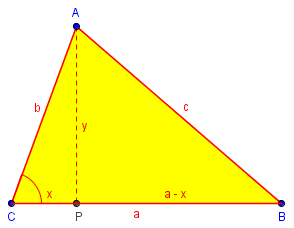
\includegraphics[width=2.5in]{img/cos} 
\end{figure}
\begin{tiny}Proof: by Pythagoras Theorem $x^2+y^2=b^2$ and $(a-x)^2+y^2=c^2$. Subtract
both equations to eliminate $y^2$ to get $c^2=a^2+b^2-2ab (x/b)$. Use the definition of the  cosine to conclude.\end{tiny}\end{frame}


\begin{frame}{Orthogonal vectors}

\textcolor{blue}{Example:} Let ${\bf u}'=(2, -1, 3)$, ${\bf v}'=(5,-4,-1)$. Then
$$
{\bf u}' {\bf v}=11\leq \vert {\bf u} \vert \, \vert {\bf v} \vert=\sqrt{14} \sqrt{42} \approx 24.24.
$$
What is the angle formed between $\bf{u}$ and $\bf{v}$?
$$
\cos ({\bf u}, {\bf v})=\frac{{\bf u}' {\bf v}}{\vert {\bf u} \vert \, \vert {\bf v}\vert}=\frac{11}{\sqrt{14} \sqrt{42}} \approx 0.4537
$$
Therefore the angle is approximately $63^{\circ}$.
\vskip 12pt
\textcolor{blue}{Definition:} Two vectors ${\bf u}, {\bf v}$ in $\R^n$ are called \textcolor{blue}{orthogonal} if
the angle they form is $90^{\circ}$. 
\vskip 12pt
Since $\cos(90^{\circ})=0$, by Properties 4. and 5. we get  that two vectors  ${\bf u}$ and ${\bf v}$ are \textcolor{blue}{orthogonal} if and only if  ${\bf u}' {\bf v}=0$ and if and only if
$$
\vert {\bf u}- {\bf v}\vert^2=\vert {\bf u} \vert^2 +\vert {\bf v}\vert^2.
$$
\end{frame}


\begin{frame}{Another proof of Cauchy-Schwarz inequality}

We want to prove that ${\bf u}' {\bf v} \leq  \vert {\bf  u} \vert \, \vert {\bf v} \vert$ for all $\bf{u}$ and $\bf{v}$ in $\R^n$.
\vskip 12pt
If $\vert \bf{u} \vert$ and/or $\vert \bf{v} \vert$ are 0 it is trivial, so we assume they are both non-zero.
\vskip 12pt
Consider  the unit vectors $\bf{w_1}=\frac{\bf{u}}{\vert \bf{u} \vert}$ and
$\bf{w_2}=\frac{\bf{v}}{\vert \bf{v} \vert}$. Then it suffices to show that  
$${\bf w_1}' {\bf w_2} \leq  1.$$


Since $\vert {\bf w_1}-{\bf w}_2 \vert^2 \geq 0$, developing this inequality  we  conclude the desired proof.
\vskip 12pt
 Observe that if both vectors are non-zero, then we have \textcolor{blue}{equality}  if and only if $\bf{u}=\lambda \bf{v}$
for some $\lambda \neq 0$, that is, the vectors are  \textcolor{blue}{co-linear}. 
\vskip 12pt
Two co-linear vectors are also called \textcolor{blue}{linearly dependent}. This notion can be  generalized to a family of $m$ vectors in $\R^n$ as follows.\end{frame}

\begin{frame}{Linear dependence and independence}


A \textcolor{blue}{linear combination} of $m$ vectors in $\R^n$ ${\bf v_1},\dots, \bf{v}_m$ is the vector in $\R^n$ defined as
$$
{\bf u}= \lambda_1{\bf  v_1}+\cdots +\lambda_m {\bf v_m}.
$$
where $\lambda_1,...,\lambda_m$ are real numbers.
\vskip 12pt
If $\lambda_i \geq 0$ for all $i=1,\dots,m$ and $\lambda_1+\cdots+\lambda_m=1$, then it is called \textcolor{blue}{convex combination}.
\vskip 12pt
$m$ vectors in $\R^n$ $\bf{v}_1,\dots, \bf{v}_m$ are said to be \textcolor{blue}{linearly dependent} if there exist real numbers $\lambda_1,...,\lambda_m$ not all zero such that
\begin{equation} \label{1}
 \lambda_1{\bf v_1}+\cdots +\lambda_m {\bf v_m}=\bf{0}.
\end{equation}
If this equation
has the only solution $\lambda_1=\cdots =\lambda_m=0$, then $\bf{v}_1,\dots, \bf{v}_m$ are said to be \textcolor{blue}{linearly independent}.
\vskip 12pt
Observe that (\ref{1}) is a \textcolor{blue}{linear system of $n$ equations and $m$ unknowns} (Chapter 8).
\end{frame}\begin{frame}{Linear dependence and independence}

\textcolor{blue}{Remark:} $\bf{v}_1,\dots, \bf{v}_m$ are \textcolor{blue}{linearly dependent} if and only if at least one of them equals a linear combination of all others.

\begin{tiny}Proof: if $\lambda_k \neq 0$, then $\bf{v}_k$ writes as  a linear combination of all others.\end{tiny}

\vskip 12pt
\textcolor{blue}{Examples:} 
\begin{enumerate}
\item The vectors ${\bf v_1}'=(3,1)$ and ${\bf  v_2}'=(-9,-3)$ are linearly dependent since $\bf{v}_2=-3\bf{v}_1$.\begin{tiny} (the line through the vectors is $y=x/3$)\end{tiny}
\vskip 11pt
\item The vectors ${\bf v_1}'=(3,1)$ and ${\bf v_2}'=(-1,2)$ are linearly independent since the system $\lambda_1 {\bf v_1}+\lambda_2 \bf{v}_2=\bf{0}$ has the unique solution $\lambda_1=\lambda_2=0$.\begin{tiny} (2 vectors are l.i. if and only if they don't lie in the same line and 3 vectors are l.i. if and only if they don't lie in the same plane) \end{tiny}
\vskip 11pt
\item The set of unit vectors $\bf{e}_1, \dots, \bf{e}_n$ in $\R^n$ forms a set of linearly independent vectors. 
\end{enumerate}\end{frame}
\begin{frame}{Vector spaces}

Any set of $n$ linearly independent vectors $\bf{v}_1,\dots, \bf{v}_n$ forms a \textcolor{blue}{basis} of $\R^n$ since any vector $\bf{u}$ in $\R^n$ writes as a linear combination of these vectors:
$$
{\bf u}=\lambda_1 {\bf v_1}+\cdots+\lambda_n {\bf v_n}. 
$$
We  say that they \textcolor{blue}{span} $\R^n$.
\vskip 12pt
The set of unit vectors $\bf{e}_1, \dots, \bf{e}_n$ in $\R^n$ is called the \textcolor{blue}{standard basis} of $\R^n$ since the scalars of the linear combination are the coordinates of $\bf{u}$.
\end{frame}

\begin{frame}{Vector spaces}




\textcolor{blue}{Theorem:} If $\bf{v}_1,\dots, \bf{v}_n$ forms a basis of $\R^n$, then every vector in $\R^n$ 
can be \textcolor{blue}{uniquely} written as a linear combination of the basis. 

\begin{tiny}Proof: Assume one vector has two different linear combination ans show that they are equal using linear independence.\end{tiny}
\vskip 12pt
\textcolor{blue}{Theorem:} Let $\bf{v}_1,\dots, \bf{v}_n$ be a basis of $\R^n$, and let a vector  $\bf{u}_k$ in $\R^n$ that writes as
$$
{\bf u_k}= \lambda_1{\bf v_1}+\cdots+\lambda_k{\bf v_k}+\cdots +\lambda_n {\bf v_n},
$$
with $\lambda_k \neq 0$. The $\bf{v}_1,\dots,\bf{v}_{k-1}, \bf{u}_k, \bf{v}_{k+1}, \dots,\bf{v}_n$ is also a basis of $\R^n$. \begin{tiny}(since $\lambda_k \neq 0$ it will span the same space) \end{tiny}
\vskip 12pt
Therefore, $\R^n$ has infinitely many basis.
\end{frame}




\begin{frame}{Vector spaces}

If we consider the  linear combinations of a set (that is, the span) of $k<n$ linearly independent vectors $\bf{v}_1,\dots, \bf{v}_k$ of $\R^n$, we obtain a smaller space than $\R^n$ called a \textcolor{blue}{subspace} of $\R^n$. We say they form a basis of this subspace of dimension $k$.
\vskip 12pt
Therefore, a \textcolor{blue}{basis of a subspace} is a set  of \textcolor{blue}{linearly independent} vectors that \textcolor{blue}{spans}  the subspace.
\vskip 12pt
If the  vectors $\bf{v}_1,\dots, \bf{v}_k$ are linearly dependent, then they span a subspace of dimension $<k$. The dimension is the maximum number of linearly independent vectors in the family.
\end{frame}

\begin{frame}{Vector spaces}



\textcolor{blue}{Examples:} 
\begin{enumerate}
\item 2 linearly independent vectors in $\R^3$ span a plane (subspace of dimension 2).
\item 1 vector in $\R^2$ spans a line (subspace of dimension 1).
\item the set of solutions to an homogeneous system  $A\bf{x}=\bf{0}$  where $A$ is $m \times n$ matrix is a subspace of $\R^n$ (Chapter 7).
\end{enumerate}
\end{frame}


\begin{frame}{Examples}

\begin{enumerate}
\item  The vectors ${\bf v_1}'=(1,0,0)$, ${\bf v_2}'=(1,2,0)$ and ${\bf v_3}'=(1,2,3)$ form a basis of $\R^3$.
The vector ${\bf u}=(3,2,1)$ writes as $$(3,2,1)=2{\bf v_1}'+\frac23{\bf v_2}'+\frac13 {\bf v_3}'.$$
Therefore, $\{\bf{u}, \bf{v}_2, \bf{v}_3\}$, $\{\bf{v}_1, \bf{u}, \bf{v}_3\}$ and $\{\bf{v}_1, \bf{v}_2, \bf{u}\}$ are also bases of $\R^3$.

\item The vectors ${\bf v_1}'=(2,1,0)$, ${\bf v_2}'=(1,-1,2)$ and ${\bf v_3}'=(0,3, -4)$ span a subspace of dimension 2 since they are linearly dependent and none is a multiple of the other. \begin{tiny}In fact, $\bf{v}_1-2\bf{v}_2=\bf{v}_3$. \end{tiny}

\item A basis of the $xy$ plane in $\R^3$ is ${\bf v_1}'=(1,2,0)$, ${\bf v_2}'=(1,3,0)$. 

\item The dimension of the subspace spanned by the vectors
${\bf v_1}'=(0,1,0,1)$, ${\bf v_2}'=(1,1,0,1)$, ${\bf v_3}'=(1,0,0,0)$
and ${\bf v_4}'=(0,-1,0,1)$ is 3. A basis of this subspace is $\{\bf{v}_1, \bf{v}_2, \bf{v}_4\}$ but not $\{\bf{v}_1, \bf{v}_2, \bf{v}_3\}$. \begin{tiny}In fact, $\bf{v}_1+\bf{v}_3=\bf{v}_2$, thus $\bf{v}_4$ cannot be replaced. \end{tiny}
\end{enumerate}\end{frame}

\begin{frame}{}
\centering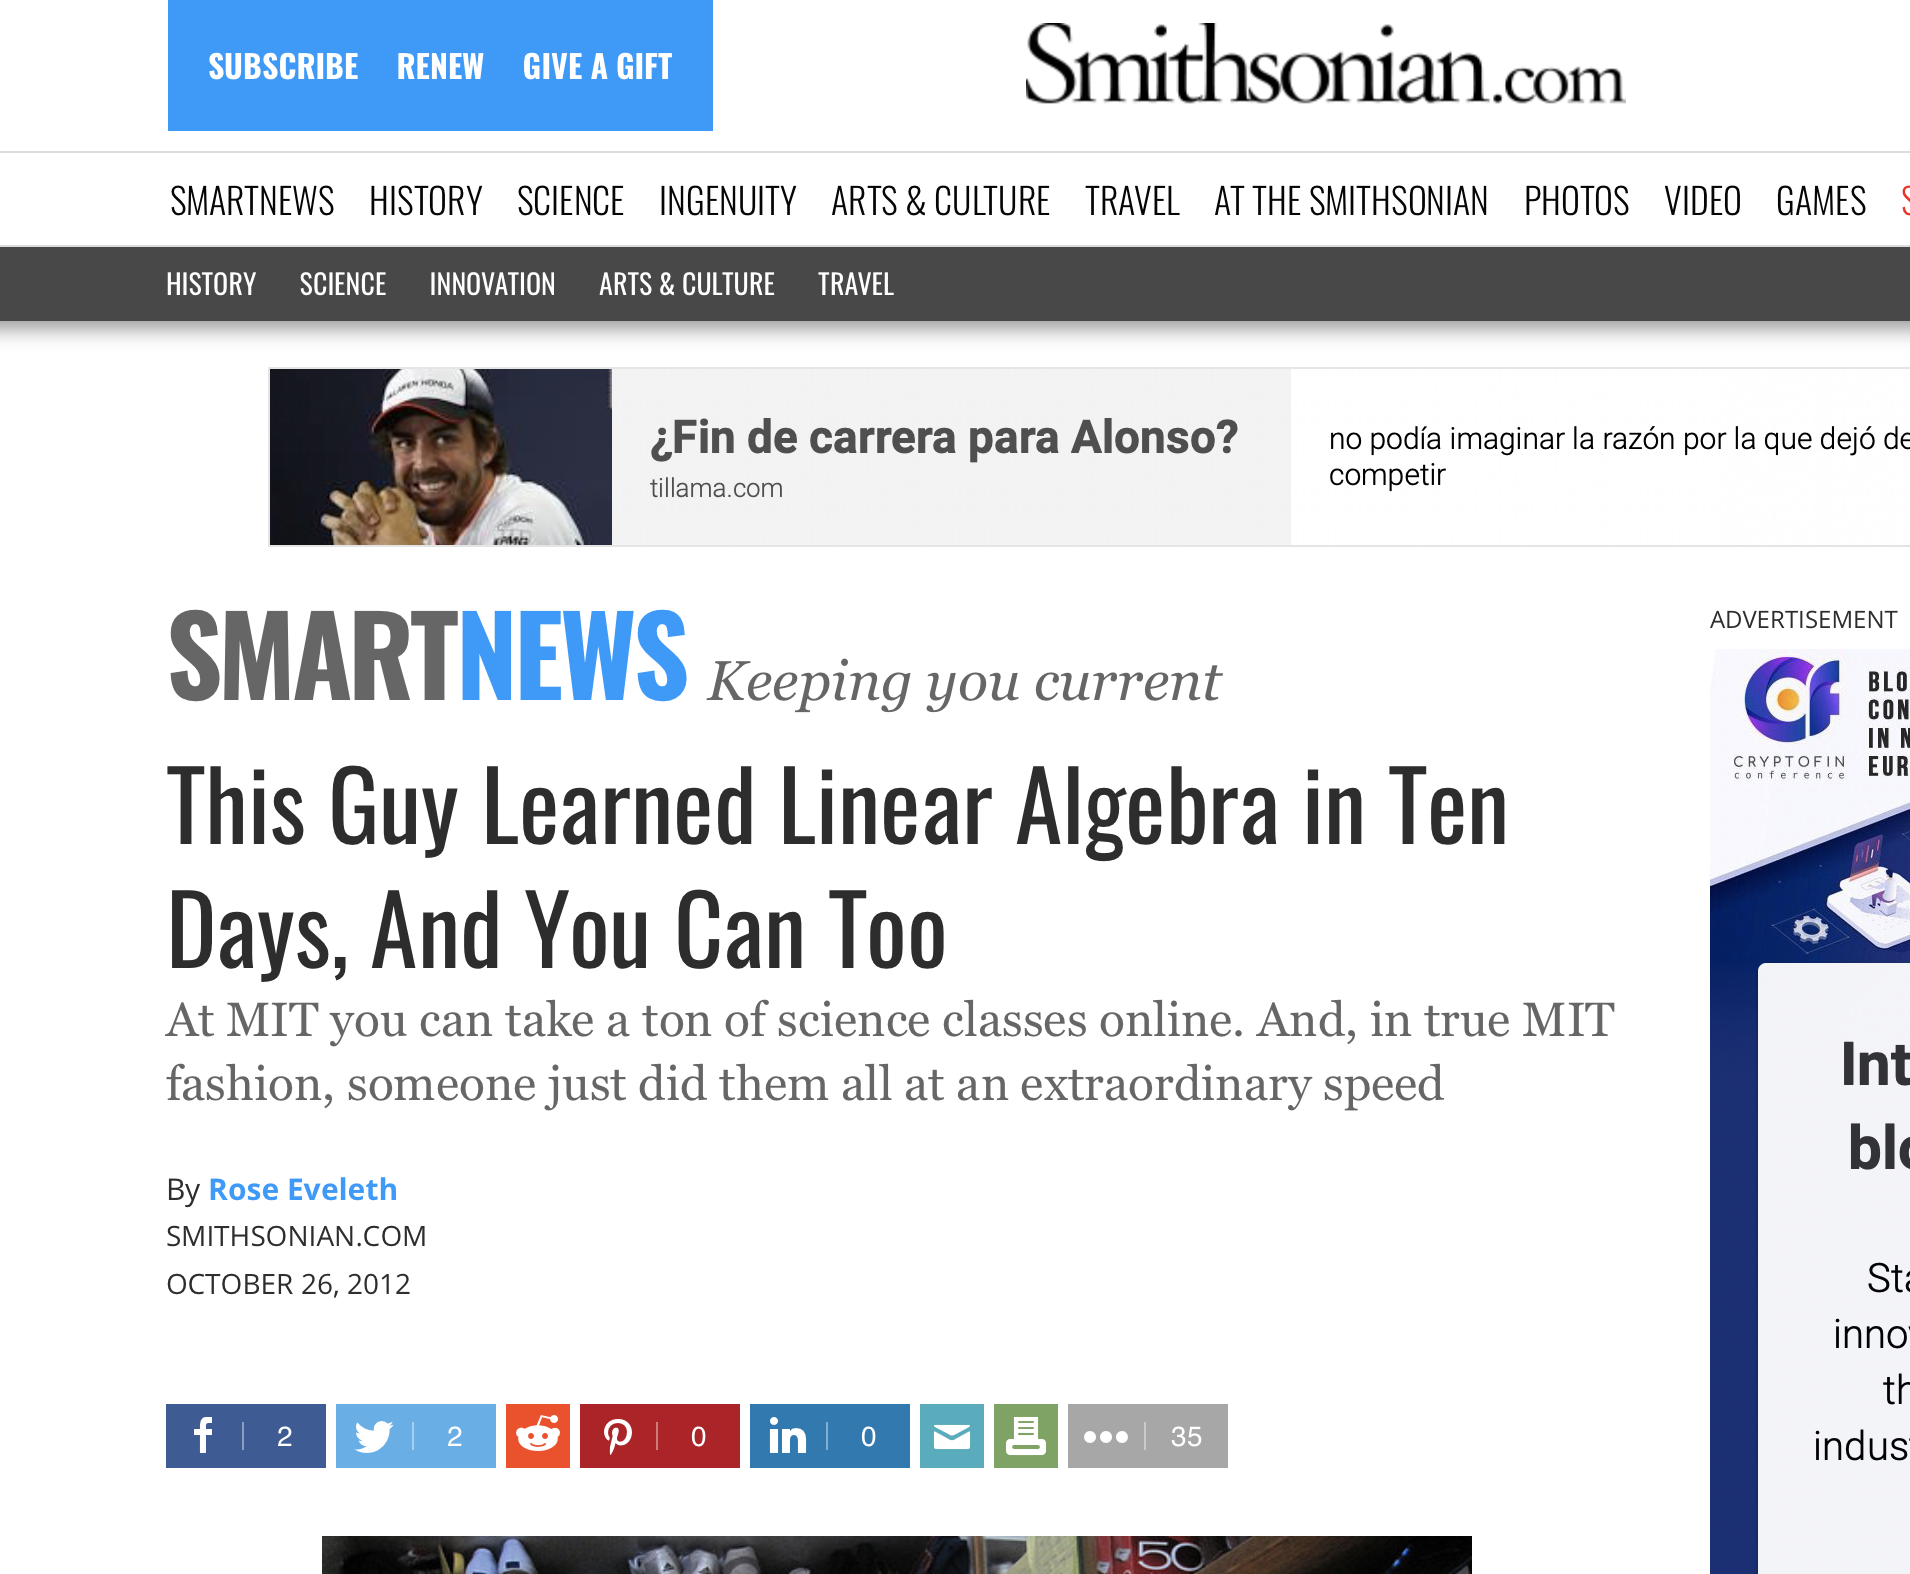
\includegraphics[height=\paperheight]{img/LinAlg10days.png}	
\end{frame}


\begin{frame}{Chapter 6: Matrices and determinants}

\textcolor{blue}{Matrices} replace the use of tables that relates two different economic units. 

\vskip 12pt
The \textcolor{blue}{operation} between matrices such as addition and multiplication simplifies the computations between the elements of different tables. 
\vskip 12pt
For example, to calculate how many units of raw material are required for the final production of a firm if some intermediate products are required.
\vskip 12pt
\textcolor{blue}{Read}  Chapter 7 of Werner-Sotskov and Chapters 8 and 9 of Simon-Blume
\vskip 12pt
\textcolor{blue}{Determinants} are useful to compute the inverse of a matrix, to solve linear equations (Chapter 7) or to find eigenvalues (Chapter 9).
\vskip 12pt
\textcolor{blue}{Exercises:} 7.6, 
7.9(b),(c),(d), 7.12, 7.14(a), 7.16, 7.18 (Werner-Sotskov)\end{frame}


\begin{frame}{Matrices}

An $m\times n$ \textcolor{blue}{matrix} is rectangular array of elements $a_{ij}$ of the form 
\begin{align*}A=(a_{ij})=\begin{pmatrix}a_{11} & a_{12} & \cdots & a_{1n}\\
a_{21} & a_{22} & \dots & a_{2n} \\
\vdots & \vdots &&\vdots \\
a_{m1}& a_{m2} &\cdots & a_{mn}
\end{pmatrix}
\end{align*}
$m$ is the number of rows, and $n$ is the number of columns and we denote by $a_{i,j}$ the entry in row $i$ and column $j$.
\vskip 12pt
If $m=n$ it is called \textcolor{blue}{square} matrix. 
\end{frame}

\begin{frame}{Matrices}


If $A$ is a $m \times n$ matrix with entries $a_{i,j}$ then its \textcolor{blue}{transpose} $A'$ is the $n\times m$ matrix with entries $a_{ji}$.
\vskip 12pt
\textcolor{blue}{Example:}
\begin{align*}A=\begin{pmatrix}2& 3 & 4 & 1\\
7 & -1 & 0 & 4
\end{pmatrix} \qquad 
A'=\begin{pmatrix}2& 7\\
3 & -1 \\
4 & 0 \\
1& 4
\end{pmatrix}
\end{align*}

A square matrix is \textcolor{blue}{symmetric} if $A'=A$ and \textcolor{blue}{antisymmetric} if $A'=-A$. 
\end{frame}


\begin{frame}{Matrices}

 A $n \times n$ \textcolor{blue}{diagonal matrix} and the \textcolor{blue}{Identity matrix} are defined respectively as
\begin{align*}D=\begin{pmatrix} d_1 & 0 & \cdots &0\\
0 & d_2 & \cdots &0 \\
\vdots & \vdots & \cdots &\vdots \\
0 &0 & \cdots &d_n
\end{pmatrix} \qquad I=\begin{pmatrix}1 & 0 & \cdots &0\\
0 & 1 & \cdots &0 \\
\vdots & \vdots & \cdots &\vdots \\
0 &0 & \cdots &1
\end{pmatrix}.
\end{align*}

 A $n \times n$ is \textcolor{blue}{upper triangular} matrix and \textcolor{blue}{lower triangular} matrix are defined respectively as
\begin{align*}U=\begin{pmatrix} u_{11} & u_{12} & \cdots &u_{1n}\\
0 & u_{22} & \cdots &u_{2n} \\
\vdots & \vdots & \cdots &\vdots \\
0 &0 & \cdots &u_{nn}
\end{pmatrix} \qquad L=\begin{pmatrix}l_{11} & 0 & \cdots &0\\
l_{21} & l_{22} & \cdots &0 \\
\vdots & \vdots & \cdots &\vdots \\
l_{n1} &l_{n2} & \cdots &l_{nn}
\end{pmatrix}.
\end{align*}

The $m \times n$ \textcolor{blue}{zero matrix} has all entries equal to zero. \end{frame}

\begin{frame}{Matrix operations}

\textcolor{blue}{Addition of matrices: }If $A=(a_{ij})$ and $B=(b_{ij})$  are $m \times n$ matrices, then the matrix
$A+B=(a_{ij}+b_{ij})$ is also $m \times n$.
\vskip 12pt
\textcolor{blue}{Multiplication by a scalar:} If $A=(a_{ij})$ is a $m \times n$ matrix and $\lambda \in \R$, then
the matrix $\lambda A=(\lambda a_{ij})$ is also $m \times n$ .
\vskip 12pt
\textcolor{blue}{Definition:} $-A=(-1)A$ and $A-B=A+(-B)$.
\vskip 12pt
The addition and scalar multiplication satisfy the usual \textcolor{blue}{commutative}, \textcolor{blue}{associative} and \textcolor{blue}{distributive} laws.\end{frame}


\begin{frame}{Matrix operations}

\textcolor{blue}{Product:} Let $A=(a_{ij})$ be a $m \times p$ matrix and $B=(b_{ij})$ a $p \times n$ matrix. Then the product $AB=(c_{ij})$ is the $m\times n$ matrix defined as
$$
c_{ij}=a_{i1} b_{1j}+a_{i2} b_{2j}+\cdots +a_{ip} b_{pj}.
$$
\textcolor{blue}{Example:}
\begin{align*}\begin{pmatrix}2& 3 & 4 & 1\\
7 & -1 & 0 & 4
\end{pmatrix} \begin{pmatrix}2& 7\\
3 & -1 \\
4 & 0 \\
1& 4
\end{pmatrix}=\begin{pmatrix}30&  15\\
15 & 66
\end{pmatrix}
\end{align*}\end{frame}


\begin{frame}{Matrix operations}

\textcolor{blue}{Properties:} 
\begin{enumerate}
\item associative: $(AB)C=A(BC)$
\item distributive: $A(B+C)=AB+AC$ and $(A+B)C=AC+BC$.
\item \textcolor{blue}{Not commutative:} $AB \neq BA$ ! 
\item If $A$ is an $n \times n$ matrix, $AI=IA=A$.

\item $(A')'=A$, $(A+B)'=A'+B'$,
$(\lambda A)'=\lambda A'$, and $$(AB)'=B'A'.$$
\end{enumerate}

\textcolor{blue}{Remark:} the matrix  $AA'$ is always square and symmetric.

\begin{tiny}Proof: $(AA')'=(A')'A'=AA'$.  \end{tiny}\end{frame}

\begin{frame}{Orthogonal matrices}

A $n \times n $ matrix $A$ is called \textcolor{blue}{orthogonal} if  $AA'=I$.
\vskip 12pt
\textcolor{blue}{Remark:} If $A$ is orthogonal, the row (and column) vectors are pairwise orthogonal and unit vectors.

\begin{tiny}Proof: The diagonal terms of $AA'$ are the square of the norm of the row and column vectors, and the non-diagonal  terms are the scalar products. \end{tiny}
\vskip 12pt
\textcolor{blue}{Example:}
\begin{align*}\begin{pmatrix}\frac{1}{\sqrt{2}}& \frac{1}{\sqrt{2}} \\
-\frac{1}{\sqrt{2}}& \frac{1}{\sqrt{2}}
\end{pmatrix} \begin{pmatrix}
\frac{1}{\sqrt{2}}& -\frac{1}{\sqrt{2}}\\
\frac{1}{\sqrt{2}}& \frac{1}{\sqrt{2}}
\end{pmatrix}=\begin{pmatrix}1&  0\\
0 & 1
\end{pmatrix}
\end{align*}
\end{frame}
\begin{frame}{Matrix operations: elementary operations}

The following columns (or row) operations in a matrix $A$ are called \textcolor{blue}{elementary operations of type 1, 2 or 3} between columns (or rows):

\begin{enumerate}


\item \textcolor{blue}{Interchange} two columns (or rows) of $A$.

\item \textcolor{blue}{Multiply} all elements of a column (or row) of $A$ by a scalar $\lambda \neq 0$.

\item \textcolor{blue}{Add} to a column (or row) the multiple of another column (or row).

\end{enumerate}\end{frame}



\begin{frame}{Determinants}

If $A$ is an $n \times n$ matrix, we denote by $A_{ij}$ the submatrix obtained from $A$ by deleting row $i$ and column $j$. Then $A_{ij}$ is a square matrix of order $(n-1) \times (n-1)$.
\vskip 12pt
 The \textcolor{blue}{determinant} of an $n \times n$ matrix $A$ is defined recursively as
\begin{equation*}
\textnormal{det}(A)=\vert A \vert=\sum_{j=1}^n (-1)^{j+1} a_{1j} \vert A_{1j} \vert.
\end{equation*}
For $n=1$ we set $\vert A \vert=a_{11}$.

\vskip 12pt
 For  $n=2$, $\vert A \vert=a_{11}a_{22}-a_{12} a_{21}$.
\vskip 12pt
For $n=3$,
\begin{equation*} \begin{split}
\vert A \vert&=a_{11} \begin{vmatrix}
a_{22}& a_{23}\\
a_{32}& a_{33}
\end{vmatrix}-a_{12}\begin{vmatrix}
a_{21}& a_{23}\\
a_{31}& a_{33}
\end{vmatrix} +a_{13} \begin{vmatrix}
a_{21}& a_{21}\\
a_{31}& a_{32}
\end{vmatrix}\\
&=a_{11} a_{22} a_{33}+a_{12}a_{23} a_{31}+a_{13} a_{21} a_{32}-a_{11} a_{23}a_{32}\\
&\qquad \qquad -a_{12} a_{21} a_{33}-a_{13}a_{22} a_{31}.
\end{split}
\end{equation*}
\end{frame}

\begin{frame}{Determinants}
A trick to remember the formula for $n=3$ is:
\begin{figure}
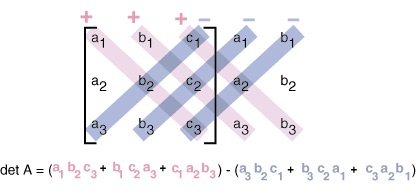
\includegraphics[width=4in]{img/deter} 
\end{figure}
\end{frame}


\begin{frame}{Determinants}

\textcolor{blue}{Theorem (cofactor expansion of a determinant):} If $A$ is an $n \times n$ matrix the determinant can be computed expanding by any row $i$:
\begin{equation*}
\vert A \vert=\sum_{j=1}^n (-1)^{i+j} a_{ij} \vert A_{ij} \vert.
\end{equation*}
or any column $j$:
\begin{equation*}
\vert A \vert=\sum_{i=1}^n (-1)^{i+j} a_{ij} \vert A_{ij} \vert.
\end{equation*}
The determinants of the submatrices $\vert A_{ij} \vert$ are called \textcolor{blue}{minors}, and the numbers  $(-1)^{i+j} \vert A_{ij} \vert$ are called \textcolor{blue}{cofactors}.
\vskip 10pt
\textcolor{blue}{Example:} Expanding by the second column:
\begin{equation*} \begin{split}
 \begin{vmatrix}
2 & 3 & 5\\
1 & 0 & 2 \\
-1 & -4 & 2
\end{vmatrix}=(-1)^3 3\begin{vmatrix}
1& 2\\
-1& 2
\end{vmatrix} + (-1)^5 (-4) \begin{vmatrix}
2 & 5\\
1 & 2
\end{vmatrix}=-16
\end{split}
\end{equation*}
\end{frame}


\begin{frame}{Determinants}

\textcolor{blue}{Properties of determinants:}
\begin{enumerate}
\item det($A$)=det($A'$).

\item If $A$ is a lower or upper triangular matrix, then the determinant equals the product of the diagonal terms.


\item An elementary operation of type 1 changes the sign of the determinant.

\item An elementary operation of type 2 multiplies the determinant by $\lambda$.

\item An elementary operation of type 3 does not change the value of the determinant.



\item  det($AB$)= det($A$)det($B$).

\item The determinant of $A$ is zero (\textcolor{blue}{singular matrix}): if two rows or columns of $A$ are equal, or if all elements of a row or columns are zero, or if a row or column is the sum of multiples of other rows or columns.

\end{enumerate}\end{frame}


\begin{frame}{Determinants}

Using Properties 2. and 5., one can compute the  determinant of any matrix by  \textcolor{blue}{Gauss elimination}.
\vskip 12pt
\textcolor{blue}{Example:} 

\begin{equation*} \begin{split}
 \begin{vmatrix}
1 & 2 & 0\\
3 & 0 & 1 \\
1 & 2 & 3
\end{vmatrix}=\begin{vmatrix}
1 & 2 & 0\\
0 & -6 & 1 \\
1 & 2 & 3
\end{vmatrix}=\begin{vmatrix}
1 & 2 & 0\\
0 & -6 & 1 \\0 & 0 & 3
\end{vmatrix}=-18
\end{split}
\end{equation*}

\begin{tiny}In the first step we have replaced $r_2$ by $r_2-3r_1$ and in the second we have replaced $r_3$ by $r_3-r_1$.\end{tiny}
\end{frame}


\begin{frame}{Determinants}

Let $A$ be a $n \times n$ matrix, $\bf{x}$ a vector (variable) in $\R^n$ and $\bf{b}$ a vector (given) in $\R^n$. Then the equation $$A\bf{x}=\bf{b}$$ is a \textcolor{blue}{linear system} of $n$ equations and $n$ variables.
\vskip 10pt
Assume that $A$ is a \textcolor{blue}{non-singular} matrix $(\vert A \vert \neq 0)$, and let $A_j(\bf{b})$ the matrix obtained replacing column $j$ of $A$ by $\bf{b}$.
\vskip 10pt
\textcolor{blue}{Cramer's rule:} The unique solution to this system is given by
$$
x_1=\frac{\vert A_1(\bf{b})\vert}{\vert A \vert}, \dots, x_n=\frac{\vert A_n(\bf{b})\vert }{\vert A \vert},
$$

\textcolor{blue}{Example:}
 \begin{equation*} 
 A=\begin{pmatrix}
2 & 3 & 5\\
1 & 0 & 2 \\
-1 & -4 & 2
\end{pmatrix}\qquad
\bf{b}= \begin{pmatrix}
1\\
7 \\
4
\end{pmatrix}
\end{equation*}
Solution: ${\bf x}'=(\frac{75}{8},-\frac{63}{16}, -\frac{19}{16})$.\end{frame}
\begin{frame}{Linear mappings}

A \textcolor{blue}{mapping} $A: \mathbb{R}^n\rightarrow \R^m$ is called \textcolor{blue}{linear} if for all ${\bf x_1},  {\bf x_2}, {\bf x} \in \mathbb{R}^n$ and $\lambda \in \R$,
$$  
A({\bf x_1}+{\bf x_2})=A({\bf x_1})+A({\bf x_2}) \quad \text{ and } \quad
A(\lambda {\bf x})= \lambda A({\bf x}).
$$

\vskip 12pt
If $A:\mathbb{R}^n\rightarrow \R^m$ is a linear mapping, then there exists an $m \times n$ matrix $A$ such that $$A({\bf x})=A {\bf x} \quad \text{for all }\quad {\bf x} \in \R^n.$$

\end{frame}

\begin{frame}{Examples of linear mappings}

\begin{enumerate}
\item Consider the linear transformation of the plane corresponding to the matrix
\begin{equation*} 
 A=\begin{pmatrix}
-1 & 0\\
0 & 1 \\
\end{pmatrix}
\end{equation*}
We have
\begin{equation*}
A\begin{pmatrix}x\\
y \\
\end{pmatrix}=\begin{pmatrix}-x\\
y \\
\end{pmatrix}.
\end{equation*}
So the mapping corresponds to the \textcolor{blue}{reflexion} across the $y$-axis.

\item The matrix of the linear transformation that \textcolor{blue}{rotates} $45^{o}$ counterclockwise any planar vector is
\begin{equation*} 
 A=\begin{pmatrix}
\frac{1}{\sqrt{2}} & -\frac{1}{\sqrt{2}}\\
\frac{1}{\sqrt{2}} & \frac{1}{\sqrt{2}} \\
\end{pmatrix}.
\end{equation*}
Observe that the first and second columns of $A$ are, respectively,
\begin{equation*}
A\begin{pmatrix}1\\
0 \\
\end{pmatrix} \quad \text{ and } \quad A\begin{pmatrix}0\\
1 \\
\end{pmatrix}.
\end{equation*}
\end{enumerate}\end{frame}




\begin{frame}{The inverse matrix}

We say that a square matrix $A$ is \textcolor{blue}{invertible} if there exists a matrix $A^{-1}$ called the \textcolor{blue}{inverse} of $A$ such that
$$
A A^{-1}=A^{-1}A=I.
$$



\textcolor{blue}{Properties:}
\begin{enumerate}
\item $(A^{-1})^{-1}=A$.
\item $(A B)^{-1}=B^{-1}A^{-1}.$
\item $(A')^{-1}=(A^{-1})'.$
\item $(\lambda A)^{-1}=\frac{1}{\lambda} A^{-1}$ if $\lambda \neq 0$.
\item $\vert A^{-1} \vert=\frac{1}{\vert A \vert}$.

\end{enumerate}\end{frame}

\begin{frame}{The inverse matrix}



\textcolor{blue}{Theorem:} A square matrix is invertible if and only if $A$ is non-singular (that is, $\vert A \vert \neq 0$).

\vskip 12pt

\textcolor{blue}{Theorem:} If $A$ is a square and non-singular matrix, then the linear system
$A{\bf x}={\bf b}$ has a unique solution given by $${\bf x}=A^{-1}{\bf b}.$$
 \end{frame}


\begin{frame}{The inverse matrix}

\textcolor{blue}{Theorem:} If $A$ is a square and non-singular matrix, then 
$$
A^{-1}=\frac{1}{\vert A \vert } ((-1)^{i+j} \vert A_{ij} \vert)',
$$ 
where $(-1)^{i+j} \vert A_{ij} \vert$ is the matrix of cofactors of $A$.
\vskip 10pt
For $n=2$, \begin{equation*}
 \begin{pmatrix}
a & b\\
c & d
\end{pmatrix}^{-1}=\frac{1}{\vert A \vert }\begin{pmatrix}
d & -b\\
-c & a
\end{pmatrix}
\end{equation*}

For $n>2$ this formula is sometimes computationally \textcolor{blue}{inefficient}. 
\vskip 10pt
In practice it is better to use \textcolor{blue}{elementary row operations} Starting form the $n \times 2n$ matrix $(A \, \vert\,  I)$,
we proceed by elementary row operations until we arrive at $(I \, \vert \, A^{-1})$.
Here only operations between ROWS are allowed (as when solving a system of equations).
\end{frame}





\begin{frame}{Input-output model}

$n$ firms produce one good each.
\vskip 10pt
$a_{ij}$=units of good $i$ needed to produce 1 unit of good $j$
\vskip 10pt
$A=(a_{ij})$ is called technology or input-output matrix.

\vskip 10pt
${\bf x}\in \R^n$ is the total amount of goods produced and ${\bf y}\in \R^n$ is the \textcolor{blue}{costumer demand} vectors of the $n$ goods.
\vskip 10pt
$A{\bf x}$ represents the \textcolor{blue}{internal demand} vector for each of the goods (units of each good to produce output of another good)
\vskip 10pt

The \textcolor{blue}{supply and demand law} tells us that the output ${\bf x}$ should be equal to the demand $A\bf{x}+{\bf y}$. We obtain the \textcolor{blue}{Input-output model}: $${\bf x}=A{\bf x}+{\bf y} \quad \Leftrightarrow \quad (I-A){\bf x}={\bf y} \quad \Leftrightarrow \quad {\bf x}=(I-A)^{-1}{\bf y},$$
if $I-A$ is invertible!\end{frame}



\begin{frame}{Input-output model}

\textcolor{blue}{Example:}  

\begin{figure}
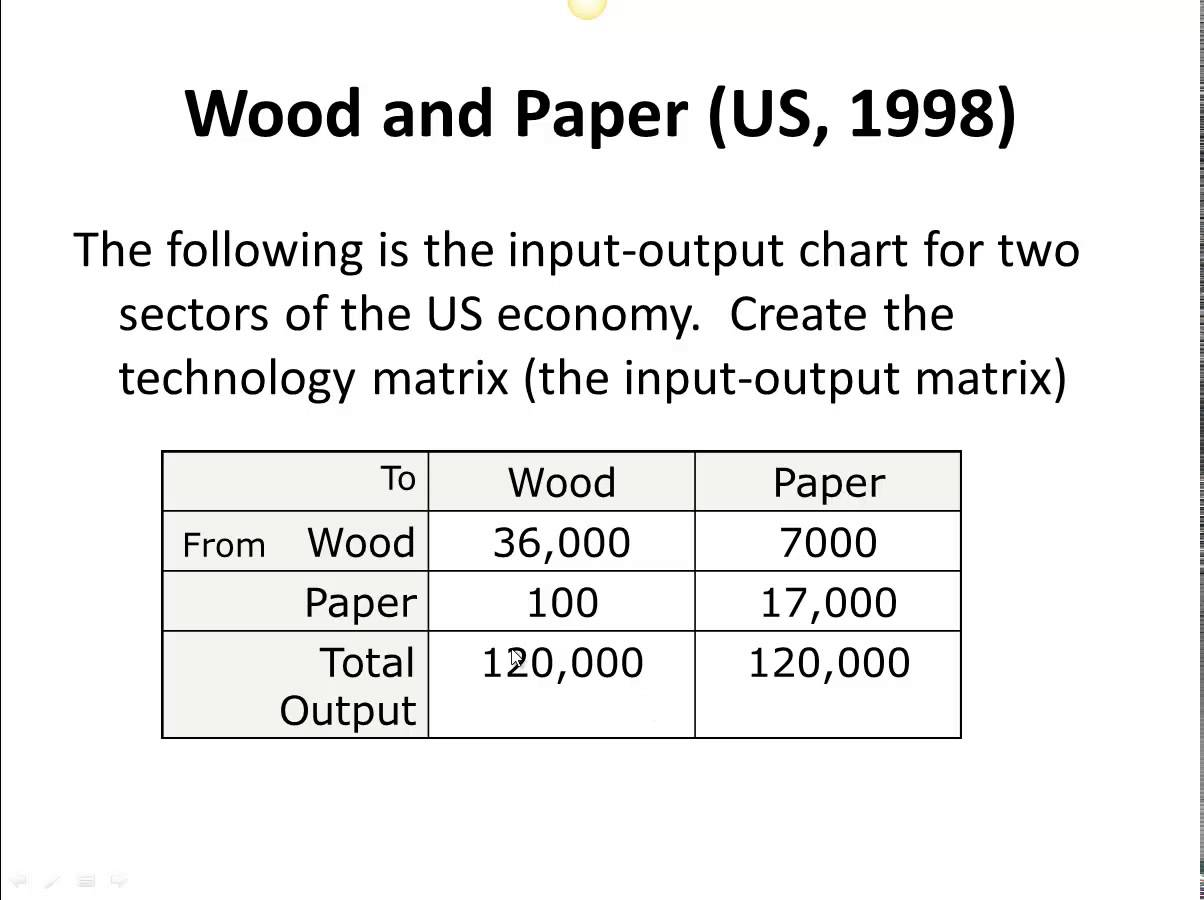
\includegraphics[width=3in]{img/io} 
\end{figure}

\textcolor{blue}{Solution:}  \begin{equation*} 
 A=\begin{pmatrix}
0.3 & 0.0583\\
0.00083 & 0.14167\\
\end{pmatrix}
\end{equation*}\end{frame}
\begin{frame}{Input-output model}

 A family of examples of $A$ is :
 \vskip 10pt
\textcolor{blue}{Theorem:} If $A$ is a square triangular matrix with all the elements of the diagonal equal to zero, then $I-A$ is invertible and
$$
(I-A)^{-1}=I+A+A^2+\cdots+A^{n-1}.
$$

\begin{tiny}Proof: check that $(I-A)(I-A)^{-1}=I$ and $(I-A)^{-1}(I-A)=I$. Use  the fact that $A^n=0$.\end{tiny}
\vskip 12pt
 \textcolor{blue}{Example:}  \begin{equation*} 
 A=\begin{pmatrix}
0 & 3 & 5\\
0 & 0 & 2 \\
0 & 0 & 0
\end{pmatrix}\qquad
\bf{y}= \begin{pmatrix}
1\\
7 \\
4
\end{pmatrix}
\end{equation*}

Solution: ${\bf x}'=(66,15, 4)$.\end{frame}
\end{document}

